\subsection{Пьезоэлектрические акселерометры}


Пьезоэлектрический метод измерения основан на использовании прямого пьезоэффекта.
Прямое пьезоэффект - явление возникновения на поверхности пьезоэлектрика за счёт электрической поляризации под действием механического напряжения.
В качестве пьезоэлектриков используются анизатропные кристаллы естественного происхождения (например \ce{SiO2}), синтетические кристаллы (сегнетова соль \ce{C4H12KNaO10}) и поляризованные поликристаллические сегнетоэлектрики (пьезокерамика).

Для описания механического напряжения используют тензор напряжений.

\begin{figure}[ht]
	\centering
	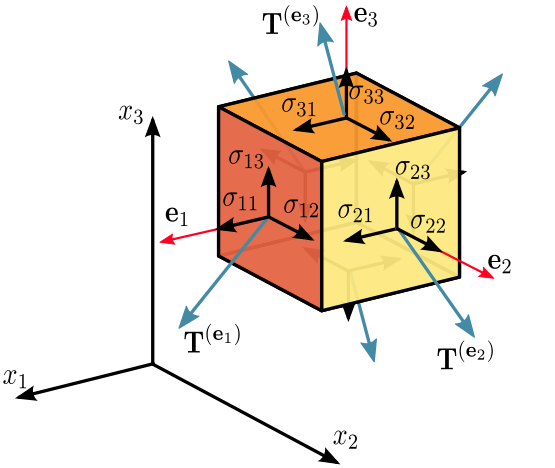
\includegraphics[width=0.5\textwidth]{images/theory/акселерометры/Тензор напряжений.png}
	\caption{Тензор напряжений}
\end{figure}

$
\mathbf{T} = 
\begin{bmatrix}
	\sigma_{11} & \tau_{12} & \tau_{13} \\
	\tau_{21} & \sigma_{22} & \tau_{23} \\
	\tau_{31} & \tau_{32} & \sigma_{33}
\end{bmatrix} = 
\begin{bmatrix}
	T_{11} & T_{12} & T_{13} \\
	T_{21} & T_{22} & T_{23} \\
	T_{31} & T_{32} & T_{33}
\end{bmatrix} = (T_{1}, T_{2}, T_{3}, T_{4}, T_{5}, T_{6})
$ \\

Одно из уравнений прямого пьезоэффекта, связывающее напряжение электрического поля и компоненты тензора механических деформаций:
\begin{equation}
	E_{i} = g_{ik} * T_{k}
\end{equation}
где $g_{ik}$ - пьезоконстанта давления.
\newpage
